\documentclass[a4paper]{article}

%% Language and font encodings
\usepackage[english]{babel}
\usepackage[utf8x]{inputenc}
\usepackage[T1]{fontenc}
\usepackage{booktabs}


%% Sets page size and margins
\usepackage[a4paper,top=3cm,bottom=2cm,left=3cm,right=3cm,marginparwidth=1.75cm]{geometry}

%% Useful packages
\usepackage{amsmath}
\usepackage{graphicx}
\usepackage[colorinlistoftodos]{todonotes}
\usepackage[colorlinks=true, allcolors=blue]{hyperref}

\def \variable {var(R)}

\title{Modelling in Biology}
\author{Monika Zbytniewska}

\begin{document}
\maketitle

\section{Population dynamics of a harvested stock of fish}
\begin{equation}
\dot{x}(t) = ax(t)
\end{equation}

\begin{equation}
\dot{x}(t) = rx(t)(1 - \frac{rx(t)^2}{k}), r>0, k>0
\end{equation}

\subsection{Show that (1) can be rewritten as (2)}


Substituting \(r = \beta y_0,  k = \frac{y_0}{\delta}\), gives: 
\[\dot{x}(t) = rx(t)(1 - \frac{rx(t)^2}{k}) = \beta y_0x(t) - \frac{\beta y_0x(t)^2}{\frac{y_0}{\delta}} \]

\[\dot{x}(t) = \beta y_0x(t) - \delta \beta x(t)^2 \beta (y_0 - \delta x(t)) x(t) = \beta y(t)x(t)\] 

\[\dot{x}(t) = ax(t)\] 

\subsection{Derive units of $\delta$, $\beta$, $r$, $k$.}

To be defined in terms of $S$, $R$ and $T$, which is the unit of species amount, the unit of resource amount and the unit of time respectively. 

\begin{itemize}
  \item $\delta$ is defined as the amount of resources, that each member of the species takes up. It's unit is therefore \(\frac{R}{S}\).
  \item $\beta$ can be derived from the equation given in the section above. \(\dot{x}(t) = \beta y(T)x(t)\). Rearranging gives \(\beta = \frac{\dot{x}}{yx}\). $\dot{x}$ is the rate of population growth, with the unit of $\frac{S}{T}$. $x(t)$ is defined as the population species at time $t$, with unit $S$ and $y(t)$ is the amount of resources available at time $t$, with unit $R$. The unit of $\beta$ is therefore \(\beta = \frac{\frac{S}{T}}{SR} = \frac{1}{TR}\). 
  \item \(r = \beta y_0\). $y_0$ has the same units as $y(t)$, which is $R$. Hence, \(r = \frac{\frac{1}{TR}}{r} = \frac{1}{T}\). It can be interpreted as a frequency. 
  \item \(k = \frac{y_0}{\delta} = \frac{R}{\frac{R}{S}} = S\). It can be interpreted as the total amount of species. 
\end{itemize}

\begin{table}[htbp]
\centering
\caption{Summary of the units}
\label{table1}
\begin{center}
    \begin{tabular}{c c c c}
    \toprule
     $\delta$ & $\beta$ & $r$ & $k$ \\ 
    \midrule
	 $\frac{R}{S}$ & $\frac{1}{TR}$ & $\frac{1}{T}$ & $S$ \\ 
    \bottomrule
    \end{tabular}
\end{center}
\end{table}


\subsection{Non-dimensionalisation}
A modified logistic growth model \(\dot(x) = rx(1 - \frac{x}{k} - qx\) should be non-dimensionalised into the form \(\frac{dz}{d\tau} = \dot{z} = z(1 - \gamma - z)\), with the substitution \(x = \lambda z\), \(t = \varepsilon \tau\). 
\[\frac{dx}{dt} = \frac{\gamma dz}{\varepsilon d\tau} = r\gamma z(1 - \frac{\gamma z }{k}) - q\gamma z\]
\[\frac{dz}{d\tau} = r\varepsilon z(1 - \frac{\gamma z}{k}) - \varepsilon qz\]
\[\frac{dz}{d\tau} = z(r\varepsilon - \varepsilon q - \frac{r\varepsilon \lambda}{k}z) \]
Find $\lambda$, $\varepsilon$, $\gamma$ in terms of $r$, $k$, $q$.
\[\varepsilon = \frac{1}{r}\]
\[\gamma = \varepsilon q = \frac{q}{r}\]
\[\frac{r\frac{1}{r}\lambda}{k} = 1\]
\[\lambda = k\]

\subsection{Units of $z$ and $\tau$}
\(x = \lambda z\), the unit of $x$ is $S$ and the unit of \(\lambda = k\) is $S$. \(t = \varepsilon \tau\) and the unit of \(\varepsilon = \frac{1}{r}\) is $T$. Therefore 
\[z = \frac{x}{k} = \frac{S}{S} = 1\] 
\[\tau = \frac{t}{\varepsilon} = \frac{T}{T} = 1\]
As seen from the units of $z$ and $\tau$, non-dimensionalisation is correct. 

\subsection{Fixed points}
The equation used for this part of the question is:
\begin{equation}
\frac{dz}{d\tau} = z(1 - \gamma - z); 
\end{equation}
\subsubsection{\(\gamma \geq 1\)}
\[0 = z(1-\gamma - z)\]
\[z_1 = 0, z_2 = 1 - \gamma\]
In this case the only physically meaningful solution ($z$ is non-negative) is \(z_1 = z_2 = 0\). 
\subsubsection{\(\gamma < 1\)}
\[z_1 = 0\]
\[z_2 = 1 - \gamma\]
In this case both $z_1$ and $z_2$ are physically meaningful for all values of \(\gamma < 1\). 

\subsection{Phase line plots}
%draw by hand and add the plots here 

\subsection{The regions of attraction of the fixed points}
The region of attraction of a fixed point is the set of points such that trajectories initialised on any of them converge to the fixed point. Phase lines sketched previously will be used for the analysis. 
\subsubsection{\(\gamma \geq 1\)}
In this case both of the fixed points are partially attractive and partially repelling. However, including the non-negative values of $z$, the points are attractive (the positive side of the phase line plot is the side of the attractive fixed points). 
\subsubsection{\(\gamma < 1\)}
Here \(z_1 = 0\) is repelling and $z_2$ is attracting.

\subsection{Long-term behaviour of the fish population}
In case where \(\gamma \geq 1\), the population decays towards zero, whilst in the case where \(\gamma < 1\), the population tends to stable non-zero size. 

\subsection{Numerical analysis using MATLAB}
The MATLAB code that was use for the purpose of the simulation is given in \ref{fig:code}. The output plots for \(\gamma = 0.5\) is shown in figure \ref{fig:0.5} and \(\gamma = 1.2\) in figure \ref{fig:1.2}. 
\begin{figure}
\centering
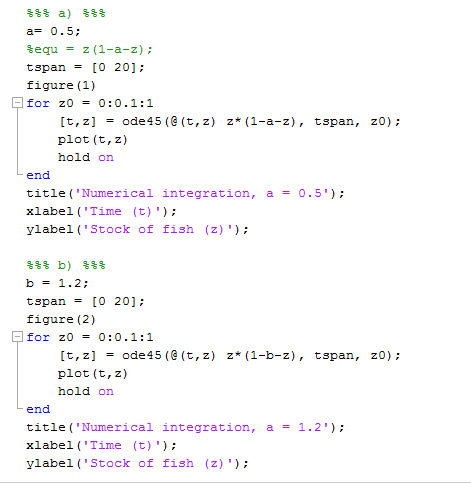
\includegraphics[width=0.5\textwidth]{code_image.PNG}
\caption{\label{fig:code}MATLAB code used to confirm the results of previous two parts.}
\end{figure}

\begin{figure}[ht]
\centering
\begin{minipage}[b]{0.45\textwidth}
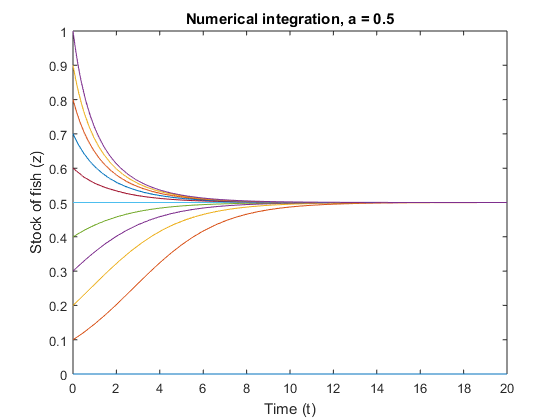
\includegraphics[width=\textwidth]{Q1_ex9_0_5.png}
\caption{\(\gamma = 0.45\)}
\label{fig:0.5}
\end{minipage}
\quad
\begin{minipage}[b]{0.45\textwidth}
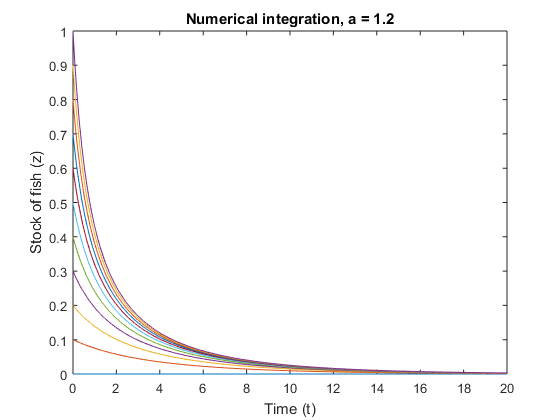
\includegraphics[width=\textwidth]{Q1_ex9_1_2.png}
\caption{\(\gamma = 1.2\)}
\label{fig:1.2}
\end{minipage}
\end{figure}

\subsection{How to maximize the amount of fish harvested per unit time?}

I'm going to use the non-dimensionalised version of the equation harvested fish equation, which already contains the variable $q$. I'm then finding derivative of the equation equal to zero, in order to find the maximum of the function. 
\[\dot{x} = rx(1 - \frac{x}{k}) - qx\]
\[\ddot{x} = r - 2x\frac{r}{k} - q = 0\]
\[q = r(1- \frac{2x}{k})\]

\pagebreak

\section{Stochastic dynamics of transcription and translation}
\subsection{$R(t)$ as a standart type of population process}
This process is known as immigration-death model, because mRNA molecules are produced at a constant rate $k_r$ and degraded at a constant rate $\gamma_r$. The master equation is given by:
\begin{equation}
\frac{dp_r}{dt} = -(k_r + \gamma_r r)p_r + k_rp_{r-1} + \gamma_r(r+1)p_{r+1}
\end{equation}

\subsection{The stationary distribution}
Applying detailed balance between $r$ and \(r+1\) gives:
\[\gamma_R(r+1)\pi_{r+1} = k_R\]
\[\frac{\pi_{r+1}}{\pi_r} = \frac{k_R}{\gamma_R (r+1)}\]
This can be expanded into:\\
\(r = 0\)
\[\pi_1 = \frac{k_R}{\gamma_R}\pi_0\]
\(r = 1\)
\[\pi_2 = \frac{k_R}{2\gamma_R}\pi_1 = {(\frac{k_R}{\gamma_R})}^2\frac{\pi_0}{2}\]
\(r = 2\)
\[\pi_3 = \frac{k_R}{\gamma_R}\pi_2 = {(\frac{k_R}{\gamma_R})}^3\frac{\pi_0}{6}\]
What can be generalized into \ref{eq5}, which is a Poisson distribution, with its normalized version in \ref{eq6}. 
\begin{equation}
\label{eq5}
\pi_r = \pi_0 {(\frac{k_R}{\gamma_R})}^r \frac{1}{r!}
\end{equation}

\begin{equation}
\label{eq6}
\pi_r = \pi_0{(\frac{k_R}{\gamma_R})}^r \frac{exp(-k_R/\gamma_R)}{x!}
\end{equation}
Normalisation constant is \(k_R/\gamma_R\). 

\subsection{Derive $<R>$ and $Var(R)$}
Following the Poisson distribution definition, the mean and variance is given by \ref{eq7}, what can be derived as follows. Let \(k_R/\gamma_R = \alpha\) in order to simplify the derivation. 
\begin{equation}
\label{eq7}
<R> = Var(R) = k_R/\gamma_R = \alpha 
\end{equation}
\[<R> = \sum_{r=0}^{\infty} r{\alpha}^r \frac{\exp{(-\alpha)}}{r!} = \exp{(-\alpha)} \sum_{r=0}^{\infty} \alpha\frac{d}{d\alpha} {\alpha}^r \frac{1}{r!} = \alpha \exp{(-\alpha)}\frac{d}{d\alpha}\sum_{r=0}^{\infty} {\alpha}^r\frac{1}{r!} = \alpha  \]
In order to calculate the variance I need to find $<R^2>$, so similarly:
\[<R^2> = \sum_{r=0}^{\infty} r^2{\alpha}^r \frac{\exp{(-\alpha)}}{r!} = \alpha^2\exp{(-\alpha)} \sum_{r=0}^{\infty} \alpha\frac{d^2}{d\alpha^2} {\alpha}^r \frac{1}{r!} + <R> = \alpha^2 + \alpha\]
Noting that \(\alpha^2\frac{d^2}{d\alpha^2}\alpha^r = r(r-1)\alpha^r\). Therefore (from the definition of variance): 
\[Var(R) = <R^2> - <R> = \alpha = <R>\]

\subsection{Probability density of decay times}
I need to define a survival probability $S(t)$, which is the probability that the molecule is still present at time $t$. The events of degradation occur at constant rate $\gamma_R$.$S(t)$ is the probability that no degradation event occurs at time $t$, it can be therefore written as:
\[\frac{dS(t)}{dt} = -\gamma_RS(t)\]
Solving this first order differential equation gives the final definition of the survival probability $S(t)$:
\begin{equation}
\label{survival}
S(t) = \exp{-\gamma_Kt}
\end{equation}
Knowing $S(t)$, I can calculate the probability density of decay times, which is the probability that an event occurs in a small $\delta t$, having not occurred within $t$ in order to find $P(t_d)$. This is: 
\[S(t) - S(t+\delta t) = - \frac{dS(t)}{dt}\delta t + \Theta(\delta t^2)\]

$\Theta$ means higher order terms, which will be ignored.Taking the limit at $\delta t \longrightarrow 0$, gives an exponential distribution: 
\[P(t) = \frac{S(t) - S(t+\delta t}{\delta t} = - \frac{dS(t)}{dt} = \gamma_R\exp(-\gamma_Rt)\]

It follows that:
\begin{equation}
P(t_d) = \gamma_R\exp(-\gamma_Rt_d)
\end{equation}

\subsection{Probability distribution $P(n|t_d)$}


$P(n|t_d)$ is the distribution for the number of protein molecules $N$ produced by a single mRNA given a lifetime $t_d$. The protein production has a constant rate $k_Q$ during $t_d$. It can be deduced that this probability distribution is in fact Poisson distribution. The Poisson distribution arises in a number of situations, one of them being a distribution obtained for the number of entities in a system if those entities are produced at a constant rate, and destroyed at a rate proportional to their total number (an immigration-death process), which is exactly the case we're considering. \\


For a point Poisson process with rate $k_Q$, the distribution of $N$ can be calculated as a function of $k_Q$ and and $t_d$. The probability of no events is just a survival probability, as in \ref{survival} and then probability of $n$ events, which follows the Poisson distribution is:
\begin{equation}
P(n|t_d) = \frac{\exp(-k_Qt_d){(k_Qt_d)}^n}{n!}
\end{equation}

\subsection{Joint probability distribution $P(n,d_t)$}

\subsection{Transition represented by each term $k_Q$ and $\gamma_Q$}
%Scan drawings!

\subsection{Proof of the stationary distribution}

\subsection{Gillespie simulation in MATLAB}
Function that performs Gillespie simulation was created first, as shown in the figures \ref{fig:gillespie part1} and \ref{fig:gillespie part2}. Then, in a separate script, $Var(R)$ was calculated and the required function plotted (figures \ref{fig:variance part1} and \ref{fig:variance part2}). The resulting plot of $Var(Q)/<Q>$ is presented in the figure \ref{fig:q2_9}. The approximate functional dependence of $Var(Q)/<Q>$ on $b$ is a linear dependence. 

\begin{figure}[ht]
\centering
\begin{minipage}[b]{0.51\textwidth}
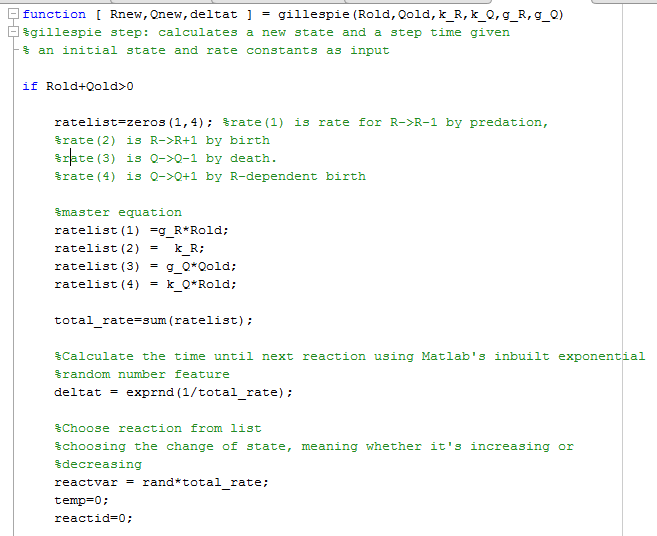
\includegraphics[width=\textwidth]{code_part1_q2.PNG}
\caption{Gillespie simulation - part 1}
\label{fig:gillespie part1}
\end{minipage}
\quad
\begin{minipage}[b]{0.39\textwidth}
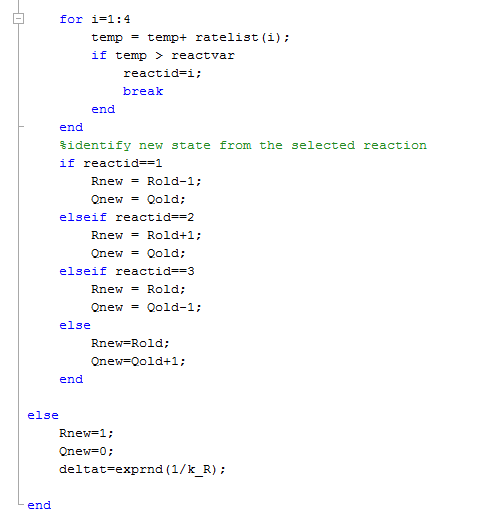
\includegraphics[width=\textwidth]{code_part2_q2.PNG}
\caption{Gillespie simulation - part2}
\label{fig:gillespie part2}
\end{minipage}
\end{figure}

\begin{figure}[ht]
\centering
\begin{minipage}[b]{0.51\textwidth}
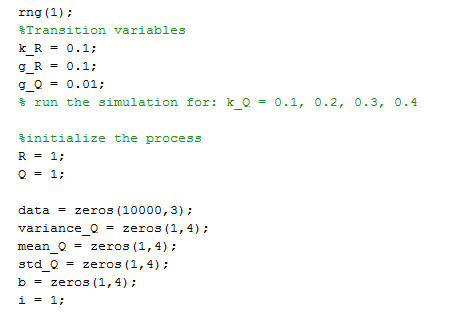
\includegraphics[width=\textwidth]{code_part3_q2.PNG}
\caption{Variance and the plot-part 1}
\label{fig:variance part1}
\end{minipage}
\quad
\begin{minipage}[b]{0.39\textwidth}
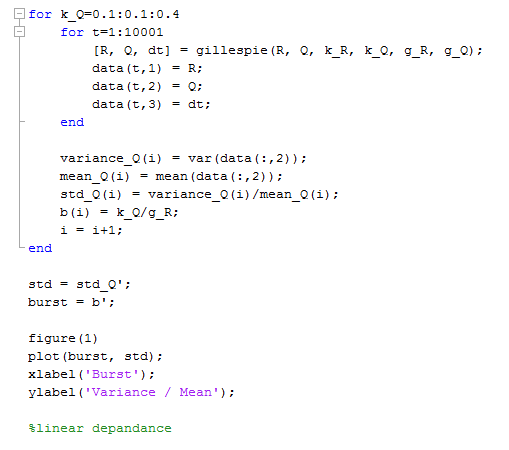
\includegraphics[width=\textwidth]{code_part4_q2.PNG}
\caption{Variance and the plot-part 2}
\label{fig:variance part2}
\end{minipage}
\end{figure}

\begin{figure}
\centering
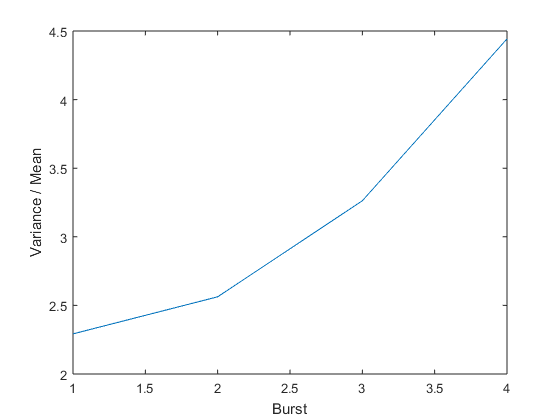
\includegraphics[width=0.5\textwidth]{q2_9.png}
\caption{\label{fig:q2_9} Plot of $Var(Q)/<Q>$ against burst size \(b = k_Q/\gamma_R\).} 
\end{figure}

\subsection{Is $Q(t)$ more or less variable relative to its mean than $R(t)$?}

In order to answer this question, the same Gillespie simulation was performed and variance calculated, but for the variable $R$. The code used to calculated $Var(R)/<R>$ is shown in figures \ref{fig:code_10 part1} and \ref{fig:code_10 part2}. Then the same dependence was plotted for both $R$ and $Q$. From figure \ref{fig:q2_10} it can be concluded that $Q(t)$ is more variable relative to its mean than $R(t)$, because the values of $variance/mean$ are larger for $Q(t)$ than for $R(t)$. 

\begin{figure}[ht]
\centering
\begin{minipage}[b]{0.48\textwidth}
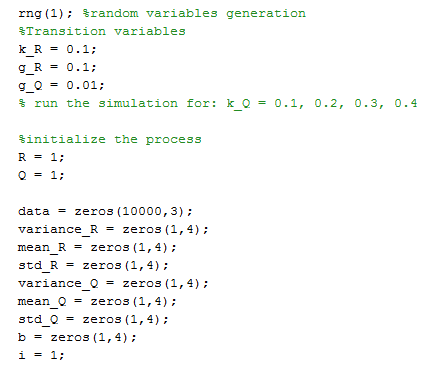
\includegraphics[width=\textwidth]{code_part1_q2_10.PNG}
\caption{$Q(t)$ and $R(t)$ - part 1}
\label{fig:code_10 part1}
\end{minipage}
\quad
\begin{minipage}[b]{0.42\textwidth}
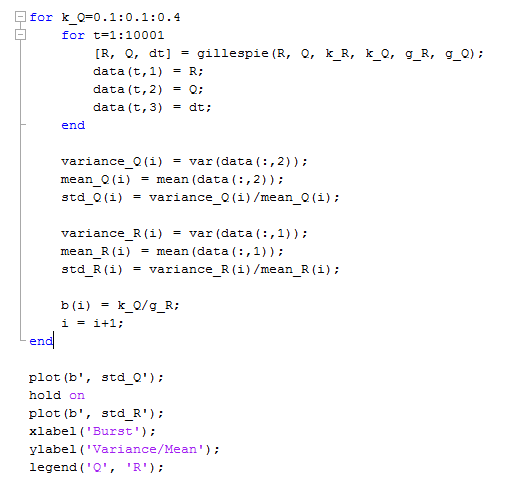
\includegraphics[width=\textwidth]{code_part2_q2_10.PNG}
\caption{$Q(t)$ and $R(t)$ - part 2}
\label{fig:code_10 part2}
\end{minipage}
\end{figure}

\begin{figure}
\centering
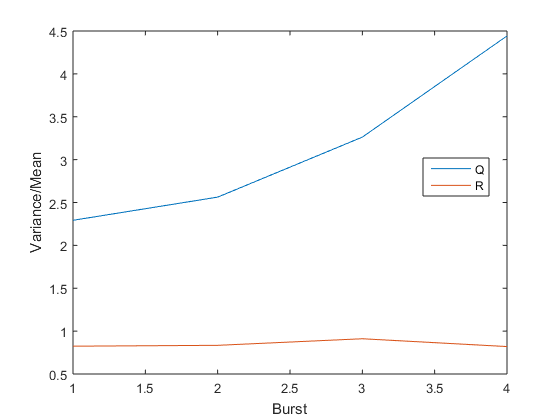
\includegraphics[width=0.5\textwidth]{q2_10.png}
\caption{\label{fig:q2_10} Plot of $Var(Q)/<Q>$ and $Var(R)/<R>$ against burst size \(b = k_Q/\gamma_R\).} 
\end{figure}

















\end{document}